\newpage
\fancyhead[C]{Rory Millard}
\section{Project Financing} \label{financing}

% --- Introduction: Clearer statement of purpose ---
This section presents an economic analysis comparing the drone-based landmine detection system proposed in this report with legacy manual metal-detector methods, focusing on the cost-effectiveness for surveying \textbf{and demining} operations near Kharkiv, Ukraine. The metric for comparison is the total cost to survey and clear one square kilometre (km²) of land, to a recall of over 90\%. The analysis links the system's financial improvement over the legacy system with sensor performance metrics $P_{sys}$ and $R_{sys}$.


\subsection{Cost Comparison} \label{subsec:cost_structures}

The capital costs of the drone-based system proposed in this report are higher than that of legacy manual techniques, which don't rely on expensive equipment, except from transportation and metal detectors. However, for each system, the operational costs are significantly higher than the upfront capital costs due to the labour intensive surveying and clearance stages. Therefore, to compare the two systems financially, only the operational costs need to be compared, as the capital costs are small in comparison. Operational costs especially dominate if the system is leased out instead of purchased.

Legacy demining operations involve a technical survey phase costing $C_\text{legacy survey} = \$305,000 \text{ per km}^2$ surveyed, followed by a clearance phase with a nominal cost of $C_\text{clearance} = \$2,940,000 \text{ per km}^2$ cleared, according to a report from the Kyiv School of Economics\footnote{\url{https://kse.ua/wp-content/uploads/2023/09/Mining-brief_Final-1.pdf}}. Manual technical surveys typically result in clearing approximately 50\% of the surveyed area, representing a precision improvement of 2$\times$ over indiscriminate 'blind' clearance. This is significantly lower than the 27.7$\times$ estimated for the proposed system in Section \ref{fusion_bounds}. The operational cost of technical survey and clearance for legacy manual methods is estimated as:
\begin{equation}
C_{\text{legacy}} = C_{\text{legacy survey}} + (0.5 \times C_{\text{clearance}}) = \$305,000 + (0.5 \times \$2,940,000) = \$1,775,000 \text{/km}^2 
\end{equation}
The operational cost associated with surveying using the proposed drone-based system needs to be estimated. Operation involves one person working 7 hours per day, which is the high thermal contrast window detailed in Section \ref{compvis_thermalsims}. The thermal drone's scanning rate is 62 m$^2$ every 5 seconds (Section \ref{thermal_selection}). Assuming radar scans can be performed approximately concurrently, the survey duration for 1 km$^2$ is estimated at $\approx$ 4 days. With an operator wage of \$15/hr, the labour cost amounts to approximately \$500/km$^2$. The cost of electricity for battery charging is considered negligible in comparison. The expected system wear and tear must also be factored in, as it represents a large operational cost. This is difficult to quantify precisely without field trials, but the cost is estimated at \$1000/km$^2$. Consequently, the total estimated operational survey cost for the drone-based system is approximately \$1500/km$^2$.

To compare the drone system with legacy methods, the cost of clearing a flagged region is assumed to depend only on the region's area. The total operational cost for the drone system $C_{\text{drone}}$, is therefore determined by the number of flagged points, which is a function of $P_\text{sys}$ and $R_\text{sys}$, as described in Section \ref{subsec:performance_savings}. Table \ref{tab:cost_comparison_structured} presents a comparison of the estimated \textbf{operational} costs.

\begin{table}[h!]
% Removed \small command
\centering
\caption{Operational Cost Comparison: Single Drone-Based System vs. Single Manual Deminer in Kharkiv, Ukraine}
\label{tab:cost_comparison_structured}
\begin{tabular}{lcc} 
\toprule
\textbf{Cost Description} & \textbf{Drone System} & \textbf{Legacy System} \\
\midrule
\multicolumn{3}{l}{}\\
Technical Survey Cost (/km²) & \$1500 & \$305,000 \\ 
Time for Technical Survey (days/km²) &  4 & 2500 \tablefootnote{\url{https://apopo.org/what-we-do/detecting-landmines-and-explosives/how-we-do-it/mine-clearance/}} \\ 
Fraction Flagged for Clearance & 3.6\% & 50\% \\ 
Cost of Clearance (/km²) & \$106,137 & \$1,470,000 \\
 \addlinespace
\textbf{Total Cost to Demine 1 km² } & \textbf{\$107,637} & \textbf{\$1,775,000}  \\
\bottomrule
\end{tabular}
\end{table}

\subsection{Financials of System Performance} \label{subsec:performance_savings}

The operational cost of the proposed system depends on the number of point flagged for mine clearance. This depends on the initial mine density $\rho_0$, and the system's precision $P_{sys}$ and recall $R_{sys}$. The fraction of land flagged for mine clearance ($A_\text{flagged}$) is:
\begin{equation}
A_{\text{flagged}} = \frac{\text{Area Flagged}}{\text{Total Area}} \approx  \frac{\rho_0 R_\text{sys}}{P_\text{sys}}. 
\label{eq:flags_fraction} % Renamed label for clarity
\end{equation}
Given the assumption that the clearance cost just depends on the size of the flagged area, the total operational cost for the drone system per km² ($C_{\text{drone}}$) is:
\begin{equation}
C_{\text{drone}}(P_\text{sys}, R_\text{sys}) = C_{\text{survey}} + A_{\text{flagged}} \times C_{\text{clearance}} 
\approx \$1480 + \left( \frac{\rho_0 R_\text{sys}}{P_\text{sys}} \right) \times \$2,940,000 
\label{eq:drone_op_cost} % New label
\end{equation}



Equation \ref{eq:drone_op_cost} demonstrates that improving $P_{sys}$ results in a large operational cost reduction by reducing the number of points flagged for mine removal. While maximizing recall $R_{sys}$ is important for safety (as discussed in Section \ref{lossmatrix}), achieving high precision is the only way the system can be economically viable. The cost savings by choosing the proposed system over legacy systems are plotted in Figure \ref{fig:financial_savings} as a function of $P_\text{sys}$ and $R_\text{sys}$. The expected region of system performance is also plotted (using the bounds from Section \ref{fusion_bounds}), indicating an \textbf{expected operational cost saving of between $\approx$ \$1.65~m - \$1.75~m per km²} surveyed, over the legacy operational cost of \$1.775~m/km². 


% --- Figure - Needs updated caption reflecting source of data/need for recalc ---
\begin{figure}[h!]
\centering
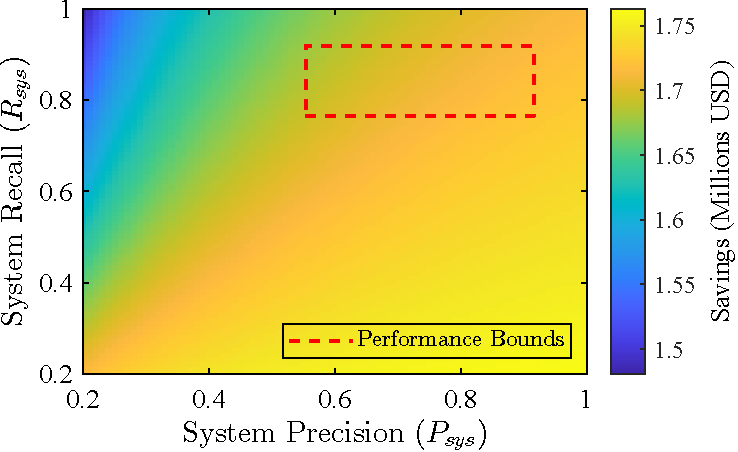
\includegraphics[width=0.5\textwidth]{figs/Rory/financial_savings.pdf} 
\caption{Plot of Equation \ref{eq:drone_op_cost}. Operational cost savings of the proposed system over legacy systems for surveying and demining 1~km$^2$, varying with $P_{sys}$ and $R_{sys}$. The expected system performance from Section \ref{fusion_bounds} is the region inside the dashed rectangle.}
\label{fig:financial_savings}
\end{figure}


\subsection{Conclusion} \label{subsec:finance_conclusion}

This section strongly suggests that the drone-based detection system proposed in this report offers significant financial benefits over legacy manual demining techniques. The operational costs are reduced by a factor of over 20$\times$, whilst the system is significantly faster. The improved precision means that the area flagged for clearance is much smaller than in legacy techniques, which causes a large reduction in the most significant part of the operational costs and times. These reductions in cost and time will enable more widespread demining operations, restoring large areas of productive land, and saving countless lives. 

Future work should investigate more accurate cost estimates. For the operational costs, more advanced YOLOv11 models (Section \ref{compvis_implementation}) should be trained on real world experimental data. The ANFIS network (Section \ref{fusion}) should be implemented, and the performance metrics $P_\text{sys}$ and $R_\text{sys}$ should be found by testing the entire system on a large dataset of unseen experimental data. This would give a more accurate picture of the system's financial viability, which would help in securing funding if the project were commercialised.

